\documentclass{article}
\usepackage[utf8]{inputenc}
\usepackage{graphicx}
\usepackage{pdfpages}
\usepackage{geometry}
\geometry{
	a4paper,
	total={170mm,257mm},
	left=20mm,
	top=20mm,
}
\title{\texttt{test\_crypto} Documentation}
%\author{Satyam Sachan}
\date{June 2022}

\begin{document}
	
	\maketitle
	
	\section{Introduction}
	The \texttt{test\_crypto} library implements the common cryptographic functions found in the Secure Hardware Extension (SHE). This document covers the construction and usage of these functions. 
	
	\section{Implemented Primitives}
	The following primitives are available as a module:
	\begin{itemize}
		\item \underline{Encryption/Decryption}: \texttt{AES-ECB} (Electronic Code Book) and \texttt{AES-CBC} (Cipher Block Chaining).
		\item \underline{Hash Function}: \texttt{Miyaguchi-Preneel Compression}.
		\item \underline{\texttt{MAC}}: \texttt{Cipher-based MAC} with \texttt{AES} as the pseudorandom function.
	\end{itemize}
	
	\subsection{\texttt{AES}}	
	The standardized cipher used for encryption/decryption and also as a subroutine where a pseudorandom function is needed.\\
	Enables the following functions:
	\begin{itemize}
		\item \texttt{CMD\_ENC\_ECB}: \texttt{ECB}-mode encryption. This function is used by the following function(s):
		\begin{itemize}
			\item \texttt{CMD\_INIT\_RNG}: Initializes the seed and derives a key for the PRNG.
			\item \texttt{CMD\_RND}: Returns a vector of 128 random bits.
			\item Memory Update Verification: Generates a verification message which can be transferred to the backend to prove the successful update.
		\end{itemize}
		\item \texttt{CMD\_ENC\_CBC}: \texttt{CBC}-mode encryption. This function is used by the following function(s):
		\begin{itemize}
			\item Memory Update: The process for memory updates (the process that calls \texttt{CMD\_LOAD\_KEY}).
			\item \texttt{CMD\_EXPORT\_RAM\_KEY}: Exports the \texttt{RAM\_KEY} into a format protected by \texttt{SECRET\_KEY}.
		\end{itemize}
		\item \texttt{CMD\_DEC\_ECB}: \texttt{ECB}-mode decryption.
		\item \texttt{CMD\_DEC\_CBC}: \texttt{CBC}-mode decryption. This function is used by the following function(s):
		\begin{itemize}
			\item \texttt{CMD\_LOAD\_KEY}: Updates an internal key of SHE.
		\end{itemize}
		\item \texttt{Miyaguchi-Preneel Compression} (referred to as M-P Compression).
		\item \texttt{Cipher-based Message Authentication Code} (referred to as CMAC).
	\end{itemize}
	
	\subsection{\texttt{Miyaguchi-Preneel Compression}}
	The M-P Compression function uses \texttt{AES-ECB} as a pseudorandom function in order to generate a hash value. \\
	Enables the following functions:
	\begin{itemize}
		\item Key derivation (referred to as KDF).
		\item \texttt{CMD\_EXTEND\_SEED}: Extend the seed and the current \texttt{PRNG\_STATE} by calling the function and supplying 128 bit of entropy.
	\end{itemize}
	\subsection{KDF}
	The key derivation function uses a key (or any other secret value) and generates another key.\\
		Enables the following functions:
	\begin{itemize}
		\item \texttt{CMD\_INIT\_RNG}.
		\item Memory Update.
		\item \texttt{CMD\_LOAD\_KEY}.
		\item \texttt{CMD\_EXPORT\_RAM\_KEY}. 
		\item Memory Update Verification.
		\item \texttt{CMD\_DEBUG}: Used to activate any internal debugging facilities of SHE. 	
	\end{itemize}
	\subsection{\texttt{CMAC}}
	The \texttt{CMAC} uses \texttt{AES-ECB} as as pseudorandom function in order to generate an authentication code.
	Enables the following functions:
	\begin{itemize}
		\item \texttt{CMD\_GENERATE\_MAC}: Generates a MAC of a given message with the help of a key.  This function is used by the following function(s):
		\begin{itemize}
			\item Memory Update.
			\item Memory Update Verification.
			\item \texttt{CMD\_EXPORT\_RAM\_KEY}. 
			\item \texttt{CMD\_DEBUG}.
		\end{itemize}
		\item \texttt{CMD\_VERIFY\_MAC}: Verifies the MAC of a given message with the help of a key identified by \texttt{KEY\_ID} against a provided MAC. This function is used by the following function(s):
		\begin{itemize}
			\item \texttt{CMD\_LOAD\_KEY}. 
			\item \texttt{CMD\_SECURE\_BOOT}: SHE verifies the MAC of the bootloader.
		\end{itemize}
	\end{itemize}
	\subsubsection*{Note}
	All the above primitives have been implemented, as have all of the above functions that have test vectors in the SHE spec.
	\subsection{Flowchart}
	The following flowchart details the relations between the functions discussed above.
	\newpage
	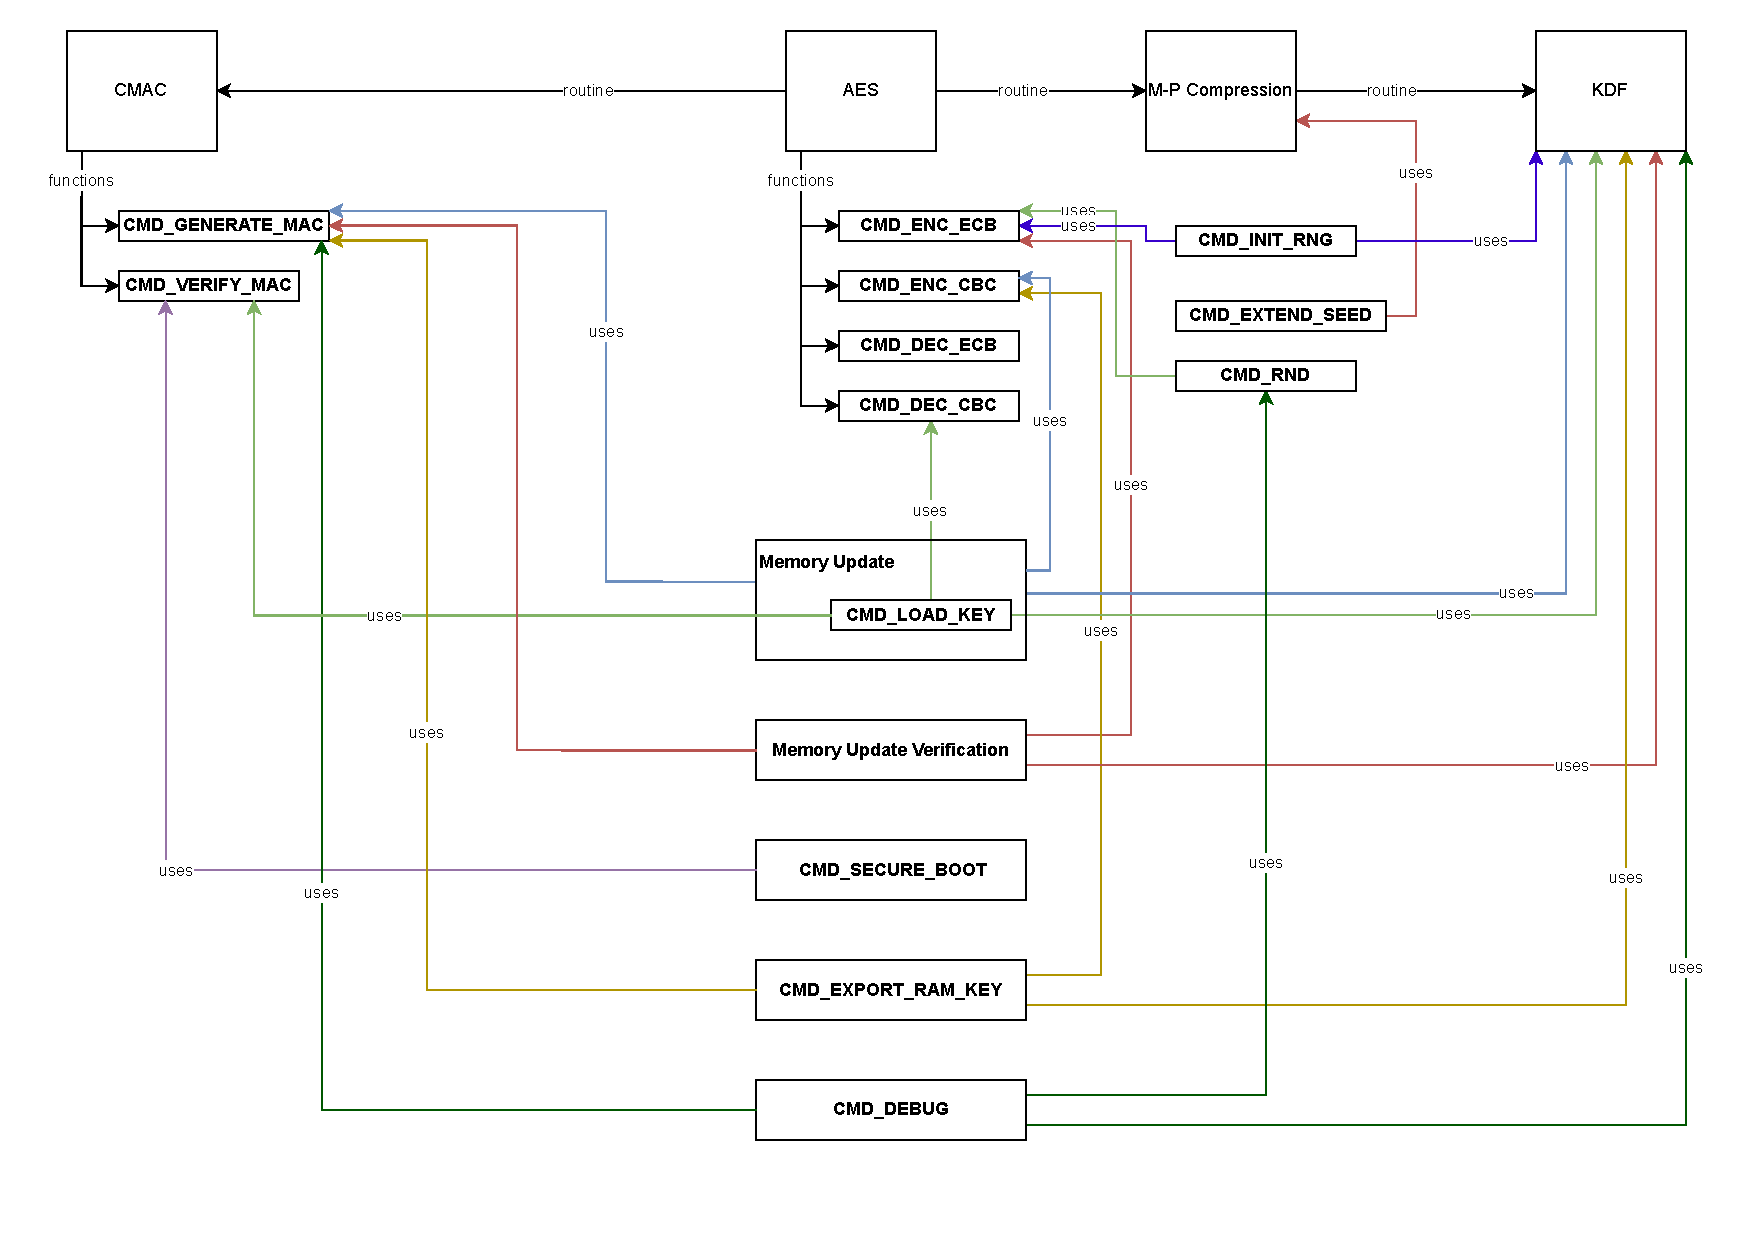
\includepdf[angle=270]{flowchart_diag.drawio.pdf}
\end{document}
